\section{Experiments and Results}
\label{sec:experiments}

We present RQ1 (incentives, Section~\ref{subsec:rq1results}), the supporting
aggregation studies (Section~\ref{subsec:supportresults}), and RQ2 (robustness on real
data, Section~\ref{subsec:rq2results}).

\subsection{RQ1: truthfulness requires an informed reference}
\label{subsec:rq1results}

Figure~\ref{fig:incentives} shows the focal agent's expected-payoff landscape as a
function of its deviation $\gamma$, one curve per number of reference substitutes $k$,
together with the profit-maximising $\gamma^\star(k)$. The pattern is exactly the one
Theorems~1--3 predict:
\begin{itemize}
    \item For $k \le 8$ the best response is pegged at the grid maximum
    ($\gamma^\star = 3$): with a poorly informed reference the focal agent profits by
    grossly over-reporting, because it can drag the reference toward its own report.
    \item At $k = 32$ the best response has fallen to $\gamma^\star \approx 1.2$ ---
    nearly truthful.
    \item For $k \ge 64$ the best response is \emph{exactly} truthful,
    $\gamma^\star = 1.0$: once the reference has enough informational substitutes, no
    deviation pays.
\end{itemize}
This is the paper's central incentive claim, realised operationally: truthful reporting
becomes a best response precisely when the reference is well-informed enough to act as
a proxy for the ground truth. As a side check, under truthful play the terminal report
reproduces the full-information Bayesian posterior to within a gap of $\sim\!10^{-13}$,
confirming the simulator implements the mechanism faithfully.

\begin{figure}[H]
    \centering
    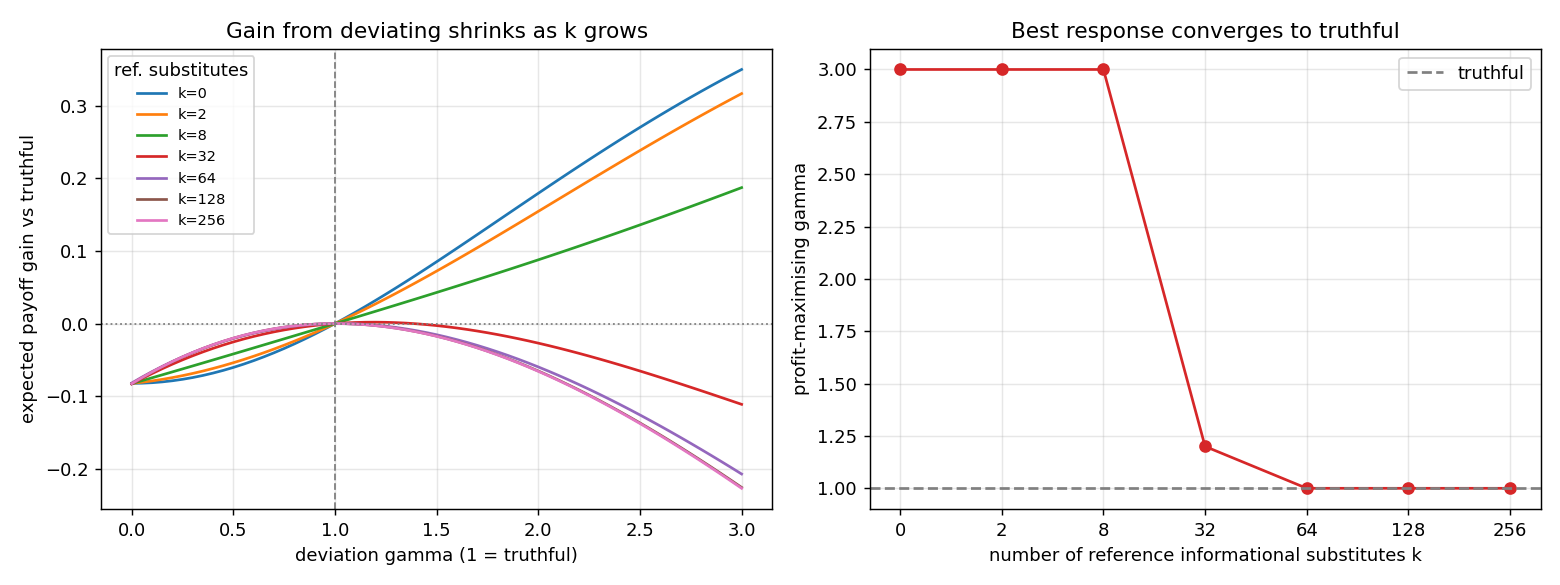
\includegraphics[width=0.95\linewidth]{Images/sim_incentives.png}
    \caption[RQ1: profit-maximising deviation vs.\ reference substitutes]{\textbf{RQ1.}
    Left: the focal agent's expected-payoff gain over truthful reporting as a function
    of its deviation $\gamma$; the gain from deviating shrinks as the reference's number
    of informational substitutes $k$ grows. Right: the profit-maximising $\gamma^\star$
    converges to the truthful value $1$ (dashed) by $k = 64$. Monte Carlo,
    $4\times 10^5$ samples per point.}
    \label{fig:incentives}
\end{figure}

\paragraph{The analytic bound $k_{\min}$.}
Figure~\ref{fig:kmin} reproduces the paper's closed-form minimum-substitutes curve. For
a stringent tolerance ($\delta = 0.1$, $\eta = 0.1$, $\varepsilon = 10^{-6}$), the bound
sits at $k_{\min} \approx 146$ substitutes and is essentially flat across the market
prior $y_1$. Two things are worth noting. First, the analytic bound is considerably
\emph{looser} than the empirical onset in Figure~\ref{fig:incentives}: the Monte Carlo
best response is already truthful at $k = 64$, whereas the worst-case bound demands
$\approx 146$ for a $10^{-6}$-small gain --- expected, since $k_{\min}$ is a worst-case
guarantee over all priors and deviations at a far tighter $\varepsilon$. Second, both
tell the same qualitative story --- the number of substitutes needed grows mildly (like
$1/(-\log(1-\delta))\cdot\log(1/\varepsilon)$) and is governed by signal
informativeness $\delta$.

\begin{figure}[H]
    \centering
    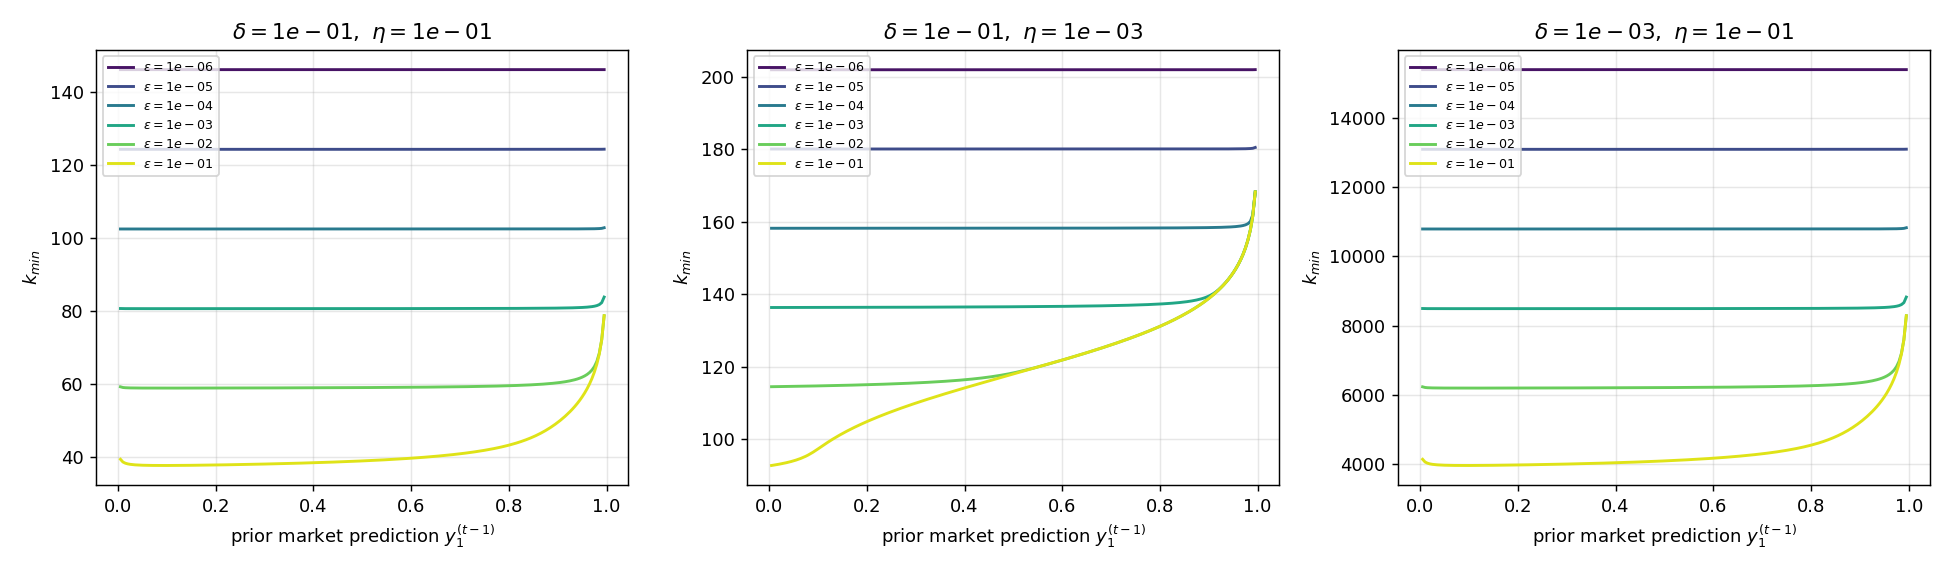
\includegraphics[width=0.8\linewidth]{Images/exp_kmin.png}
    \caption[Analytic minimum informational substitutes $k_{\min}$]{Analytic
    minimum-substitutes bound $k_{\min}$ as a function of the market prior $y_1$,
    reproducing Figure~2 of \textcite{srinivasan2025selfresolving} by chaining their
    Theorem~1, Theorem~5, and Remark~3. The bound is a worst-case guarantee and is
    looser than the empirical onset of truthfulness in Figure~\ref{fig:incentives}.}
    \label{fig:kmin}
\end{figure}

\subsection{Supporting studies: aggregation behaviour}
\label{subsec:supportresults}

\paragraph{Exact aggregation under truthful play.}
With all agents truthful, the terminal report equals the full-information Bayesian
posterior up to machine precision: the measured gap is $\sim\!10^{-16}$ across signal
qualities and market sizes. Accuracy rises with both the number of agents and signal
quality --- e.g.\ with quality $q = 0.8$ a $12$-agent market reaches $98.7\%$ accuracy,
and with weak signals $q = 0.65$ a $30$-agent market still reaches $95.4\%$. The
mechanism aggregates exactly, as claimed.

\paragraph{A few near-oracles pin the aggregate.}
Table~\ref{tab:groundtruth} shows that the reference does not need many oracles to be a
good proxy for the truth. A \emph{single} near-oracle agent (reliability $0.99$) among
$12$ raises market accuracy from $56\%$ to $99\%$, and once roughly five of twelve
agents are near-oracles the market is essentially perfect. This is the aggregation-side
analogue of RQ1's incentive result: ``enough good information in the reference'' is a
mild requirement in practice.

\begin{table}[H]
    \centering
    \caption[Value of near-oracle agents]{Market accuracy and Brier score as the number
    of near-oracle agents (reliability $0.99$) in a $12$-agent market grows. A single
    oracle already nearly resolves the market.}
    \label{tab:groundtruth}
    \begin{tabular}{cccc}
        \toprule
        \# near-oracles & oracle fraction & accuracy & Brier \\
        \midrule
        0  & 0.00 & 0.561 & 0.244 \\
        1  & 0.08 & 0.990 & 0.0097 \\
        2  & 0.17 & 0.992 & 0.0046 \\
        3  & 0.25 & 0.999 & 0.0007 \\
        5  & 0.42 & 1.000 & $\sim\!10^{-8}$ \\
        12 & 1.00 & 1.000 & $\sim\!10^{-22}$ \\
        \bottomrule
    \end{tabular}
\end{table}

\paragraph{Mixed and strategic populations.}
Table~\ref{tab:strategies} stress-tests aggregation when not everyone is truthful.
Herders, noisy reporters, and uninformative agents all degrade accuracy and open a gap
to full information, as expected. The most telling row is \texttt{uninformative\_third}:
when a third of agents report uninformatively, the designer's total cost collapses to
$0.046$ --- the mechanism \emph{pays almost nothing in the uninformative regime}, the
empirical counterpart of the paper's claim that it pays zero in uninformative
equilibria. Over-reporting, by contrast, is expensive for the designer (cost $0.506$)
while barely improving accuracy, which is the flip side of the RQ1 incentive to
over-report when the reference is weak.

\begin{table}[H]
    \centering
    \caption[Mixed-population behaviour]{Aggregate accuracy, gap to the full-information
    posterior, and designer cost across populations. The uninformative population pays
    almost nothing; over-reporting is costly without improving accuracy.}
    \label{tab:strategies}
    \begin{tabular}{lcccc}
        \toprule
        population & accuracy & Brier & gap to full-info & mean total cost \\
        \midrule
        all truthful        & 0.845 & 0.105 & $\sim\!10^{-16}$ & 0.341 \\
        half herders        & 0.768 & 0.154 & 0.164 & 0.197 \\
        noisy               & 0.703 & 0.230 & 0.244 & 0.380 \\
        uninformative third & 0.642 & 0.213 & 0.279 & \textbf{0.046} \\
        overconfident       & 0.852 & 0.112 & 0.074 & \textbf{0.506} \\
        \bottomrule
    \end{tabular}
\end{table}

\subsection{RQ2: do self-resolving payouts track verifiable payouts on real data?}
\label{subsec:rq2results}

\paragraph{Reference sweep.}
Table~\ref{tab:refsweep} and Figure~\ref{fig:refsweep} report agreement between the
self-resolving and verifiable payment schemes across $91$ resolved Polymarket markets,
as the reference is moved from near-resolution (\texttt{lead\_1h}) to mid-life
(\texttt{life\_50pct}). At a genuinely late reference the two schemes are almost
indistinguishable: at \texttt{lead\_24h} the median Pearson correlation of per-reporter
payouts is $1.00$, the Spearman rank correlation is $0.997$, the top-decile earners
overlap perfectly, and the designer's total payout is $95\%$ of the verifiable total.
As the reference moves earlier, the \emph{amounts} keep tracking (Pearson stays
$\ge 0.95$) but the \emph{ranking} of who earns most degrades sharply (Spearman falls to
$0.58$ at mid-life) and the total payout ratio drops to $0.56$. That degradation
\emph{is} the outcome-leakage channel: a near-resolution reference rewards exactly the
traders the outcome would, whereas a genuinely forecast-only reference cannot.

\begin{table}[H]
    \centering
    \caption[Reference sweep on Polymarket data]{Median agreement between self-resolving
    and verifiable payouts across $91$ resolved Polymarket markets, by reference. Pearson
    asks whether payout \emph{amounts} agree; Spearman whether the \emph{ranking} of
    earners agrees; ratio is self-resolving total payout over verifiable total.}
    \label{tab:refsweep}
    \begin{tabular}{lccccc}
        \toprule
        reference & Pearson & Spearman & top-decile Jaccard & payout ratio & argmax match \\
        \midrule
        \texttt{lead\_1h}      & 1.000 & 1.000 & 1.00 & 0.978 & 0.956 \\
        \texttt{lead\_24h}     & 1.000 & 0.997 & 1.00 & 0.953 & 0.923 \\
        \texttt{lead\_168h}    & 0.998 & 0.988 & 0.93 & 0.847 & 0.813 \\
        \texttt{life\_50pct}   & 0.954 & 0.581 & 0.56 & 0.559 & 0.780 \\
        \texttt{window\_1-24h} & 1.000 & 0.997 & 1.00 & 0.957 & 0.923 \\
        \bottomrule
    \end{tabular}
\end{table}

\begin{figure}[H]
    \centering
    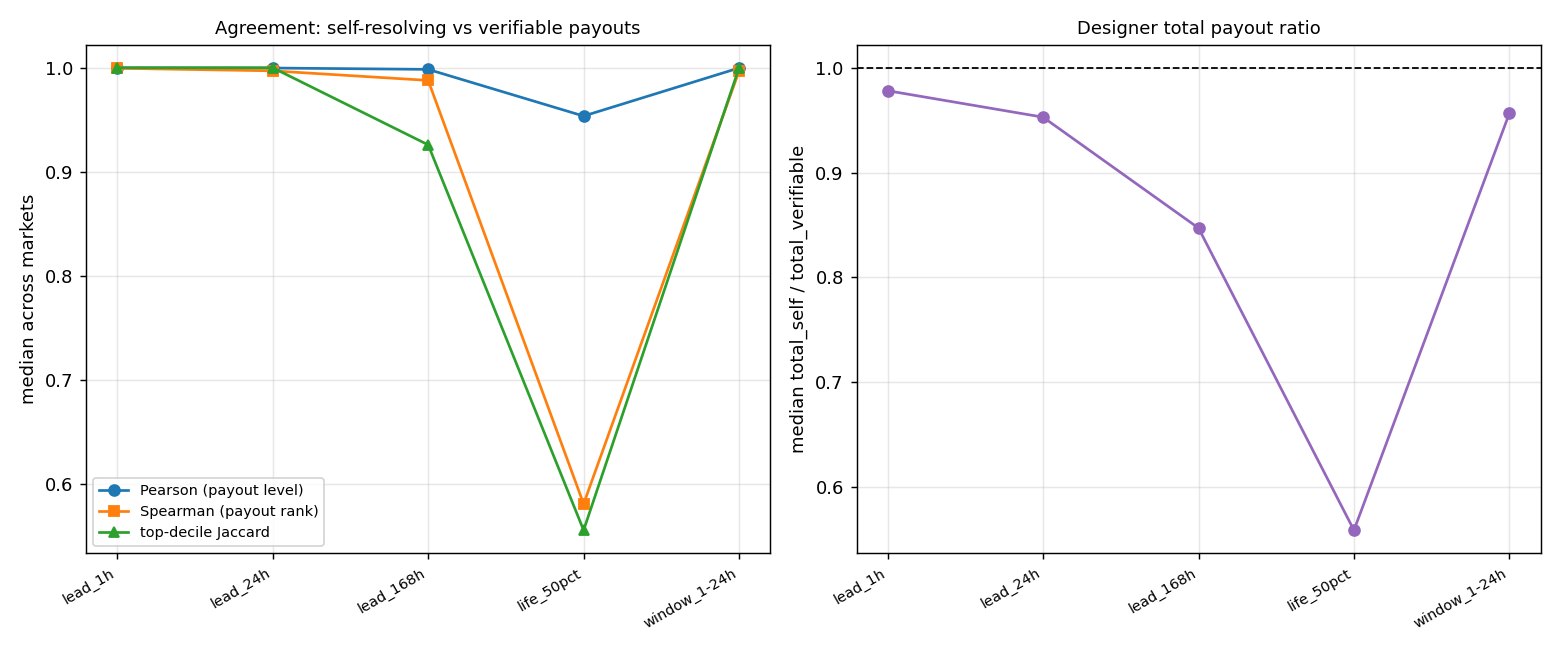
\includegraphics[width=0.85\linewidth]{Images/emp_reference_sweep.png}
    \caption[RQ2: agreement vs.\ reference lateness]{\textbf{RQ2, reference sweep.}
    Agreement between self-resolving and verifiable payouts as the reference moves from
    mid-life toward resolution. Amounts (Pearson) track throughout; ranking (Spearman)
    and the designer's total cost (ratio) are what the outcome-leakage channel inflates
    near resolution.}
    \label{fig:refsweep}
\end{figure}

\paragraph{Relative-time sweep.}
Because markets differ enormously in duration, Figure~\ref{fig:fracsweep} sweeps the
reference by \emph{relative} time to close. Agreement rises monotonically as the
reference approaches resolution: Pearson $0.94 \to 1.00$, Spearman $0.67 \to 1.00$, and
payout ratio $0.48 \to 0.94$ as we move from $90\%$-before-close to $1\%$-before-close.
The key honest takeaway is the left end of this curve: even at a genuinely \emph{early}
reference the payout \emph{levels} still track well (Pearson $\approx 0.94$); it is the
\emph{ranking} and the designer's total cost that depend on how much the reference has
already absorbed the outcome.

\begin{figure}[H]
    \centering
    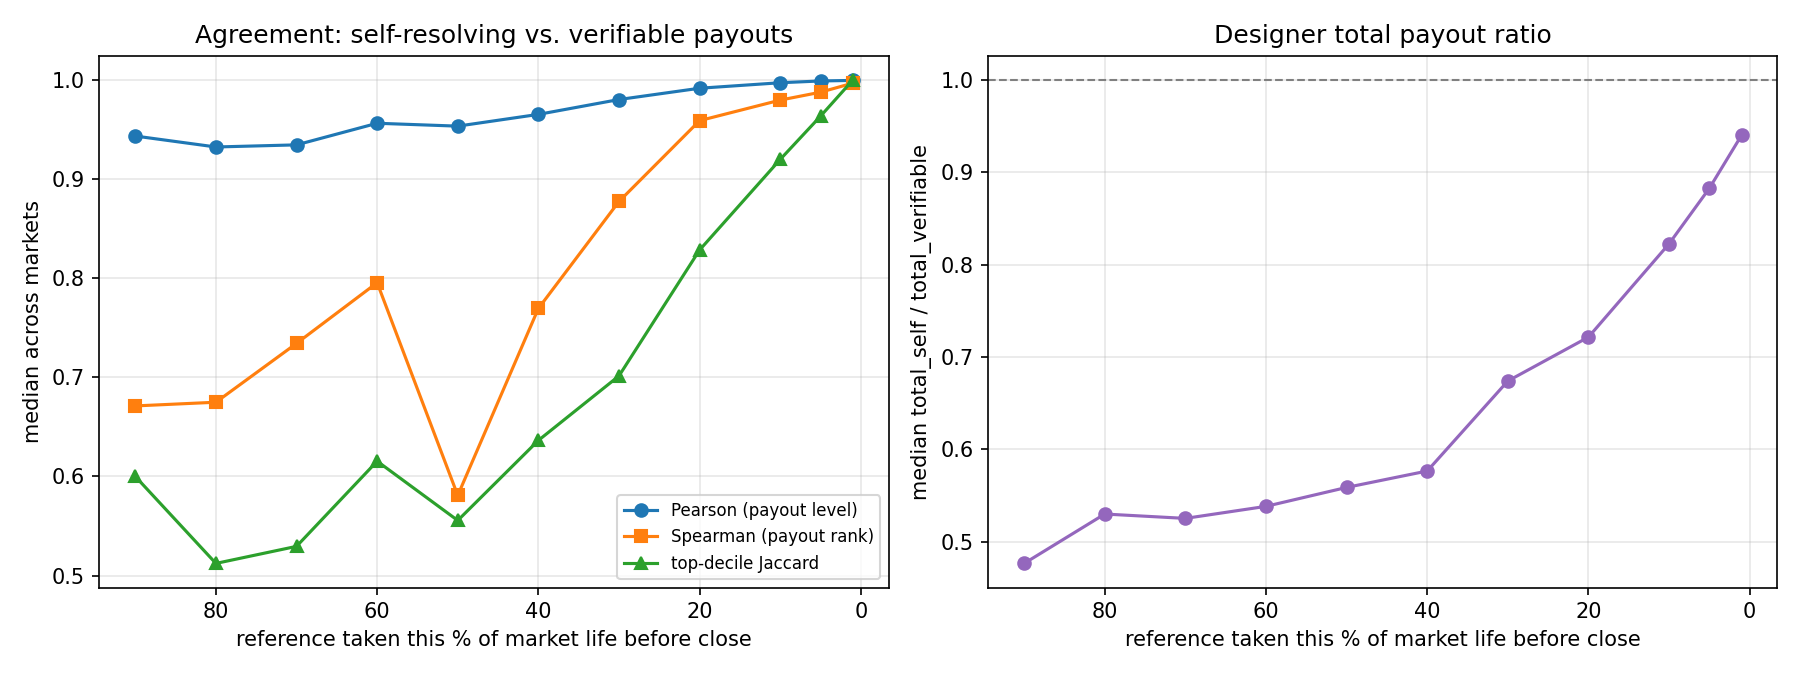
\includegraphics[width=0.9\linewidth]{Images/emp_fraction_sweep.png}
    \caption[RQ2: agreement vs.\ relative time to close]{\textbf{RQ2, relative-time
    sweep.} Median agreement as the reference is placed from $90\%$ before close (very
    early) to $1\%$ before close (near resolution). All three measures improve as the
    reference approaches resolution.}
    \label{fig:fracsweep}
\end{figure}

\paragraph{Worked example and per-market detail.}
Figure~\ref{fig:kamala} shows a representative high-volume market (the Kamala Harris
popular-vote market, $\sim\!2{,}700$ price moves, outcome $Y=0$): the self-resolving
payouts (CE-MSR against the $24$h reference) and the verifiable payouts are visually
indistinguishable (Pearson $1.00$, Spearman $1.00$, payout ratio $0.99$).
Table~\ref{tab:permarket} makes the heterogeneity explicit. At a genuinely \emph{late}
reference every market tracks perfectly; at \emph{mid-life}, some markets still track
well (the Russia--Ukraine ceasefire and Poilievre markets), while others collapse and
even invert (the US government shutdown and TikTok-ban markets, Spearman $-0.48$ and
$-0.54$). The more a late price already leaks the outcome, the larger the mid-life gap
--- and topic breakdowns reflect this too (e.g.\ sports markets, which sit flat and then
jump, keep high Pearson but low mid-life Spearman).

\begin{figure}[H]
    \centering
    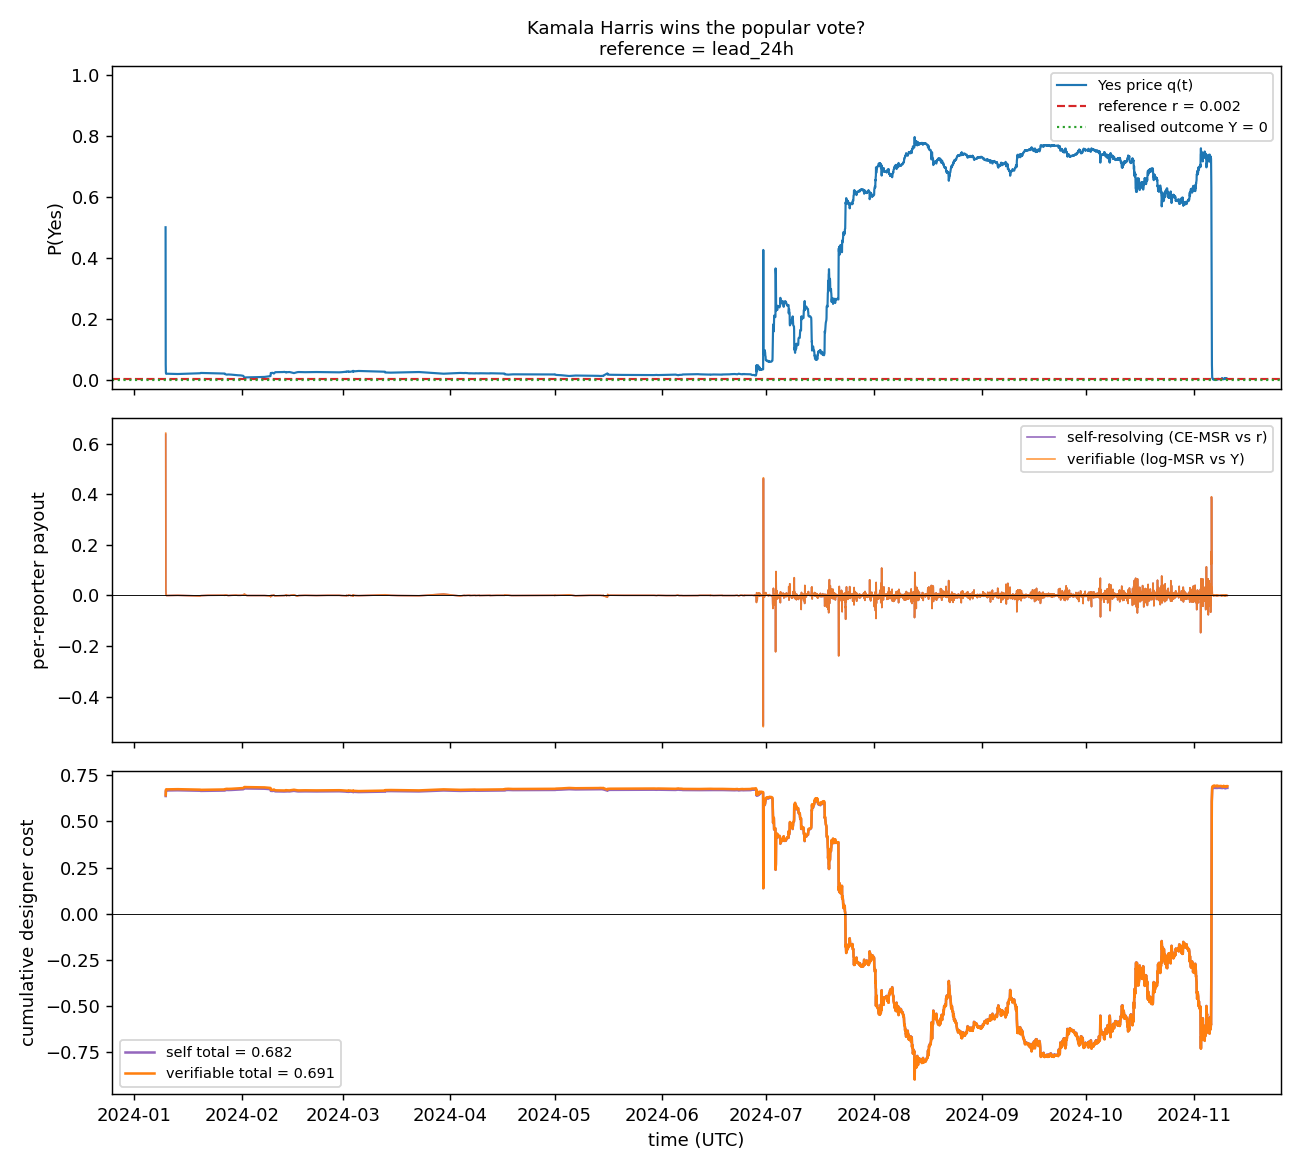
\includegraphics[width=0.85\linewidth]{Images/emp_example_kamala.png}
    \caption[RQ2: worked example]{\textbf{RQ2, worked example.} Per-reporter payouts for
    the Kamala Harris popular-vote market under the self-resolving scheme (vs.\ a $24$h
    reference) and the verifiable scheme (vs.\ the outcome). The two are nearly
    identical (Pearson $1.00$, ratio $0.99$).}
    \label{fig:kamala}
\end{figure}

\begin{table}[H]
    \centering
    \caption[Per-market agreement]{Pearson (P) and Spearman (S) correlation of
    per-reporter payouts for five high-volume markets, at a late ($24$h before close)
    and a mid-life ($50\%$) reference. Late references track perfectly; mid-life
    references track only when the late price has not yet leaked the outcome.}
    \label{tab:permarket}
    \begin{tabular}{lccccc}
        \toprule
        & & \multicolumn{2}{c}{late ($24$h)} & \multicolumn{2}{c}{mid-life ($50\%$)} \\
        \cmidrule(lr){3-4}\cmidrule(lr){5-6}
        market & \# reporters & P & S & P & S \\
        \midrule
        Kamala popular vote          & 2681 & 1.00 & 1.00 & 1.00 & 0.45 \\
        Poilievre next Canadian PM   & 1030 & 1.00 & 1.00 & 0.96 & 0.91 \\
        Russia--Ukraine ceasefire '25 & 2531 & 1.00 & 1.00 & 0.99 & 0.98 \\
        US government shutdown       &  778 & 1.00 & 1.00 & 0.41 & $-0.48$ \\
        TikTok ban (May '25)         & 1078 & 1.00 & 1.00 & $-0.37$ & $-0.54$ \\
        \bottomrule
    \end{tabular}
\end{table}

\paragraph{Summary of RQ2.}
On real data the self-resolving mechanism reproduces the verifiable mechanism's payouts
almost exactly when the reference is genuinely late, and degrades gracefully and
interpretably as the reference moves earlier. The residual gap is concentrated in the
\emph{ranking} of earners and the designer's \emph{total cost}, and is driven by
outcome leakage rather than by the mechanism failing to identify good forecasts ---
the payout \emph{levels} track even at early references.
